\label{sec:dataRange}

\begin{figure}[htp]
\centering
\frame{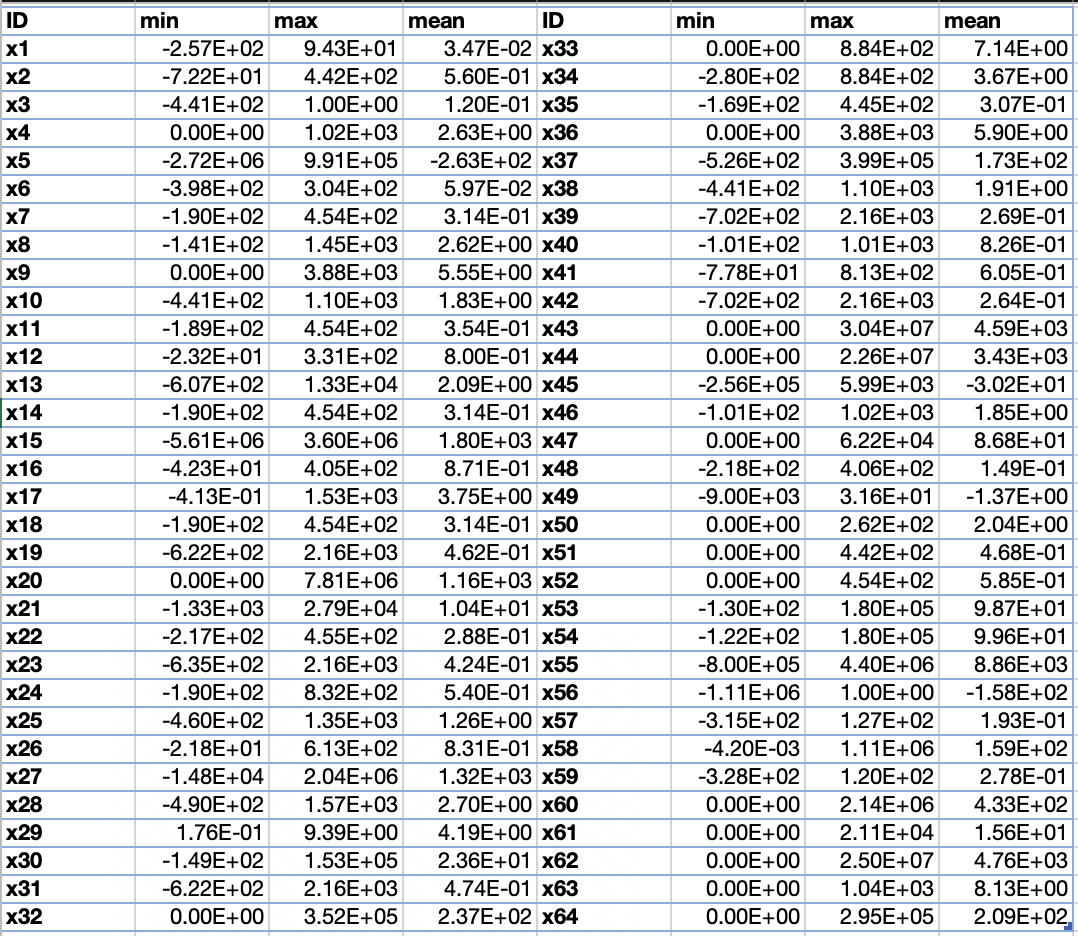
\includegraphics[width=\columnwidth]{Images/y1mmm.png}}
\caption{Min, Max and Mean for Year 1 }
\label{fig:y1mmm}
\end{figure}

% \label{sec:dataRange}
\begin{figure}[htp]
\centering
\frame{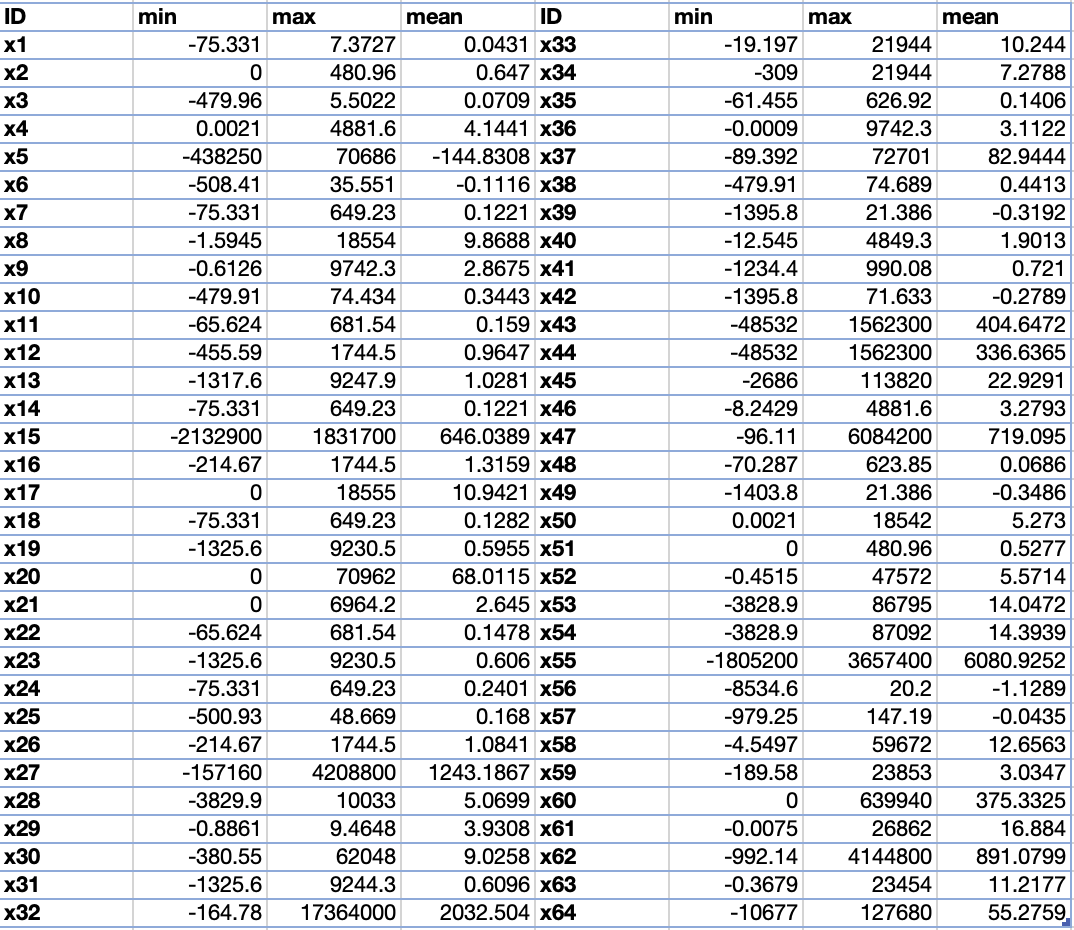
\includegraphics[width=\columnwidth]{Images/y2mmm.png}}
\caption{Min, Max and Mean for Year 2 }
\label{fig:y1mmm}
\end{figure}

% \label{sec:dataRange}
\begin{figure}[htp]
\centering
\frame{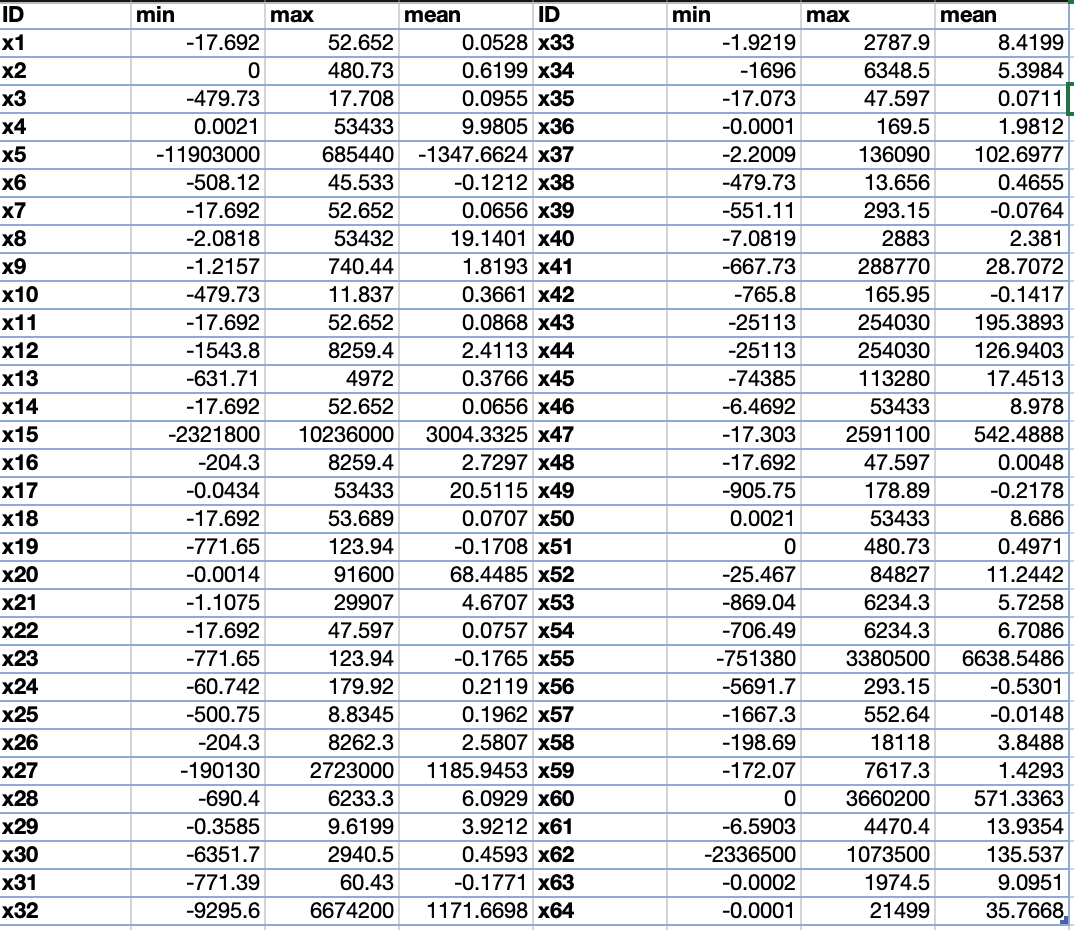
\includegraphics[width=\columnwidth]{Images/y3mmm.png}}
\caption{Min, Max and Mean for Year 3 }
\label{fig:y1mmm}
\end{figure}


\begin{figure}[htp]
\centering
\frame{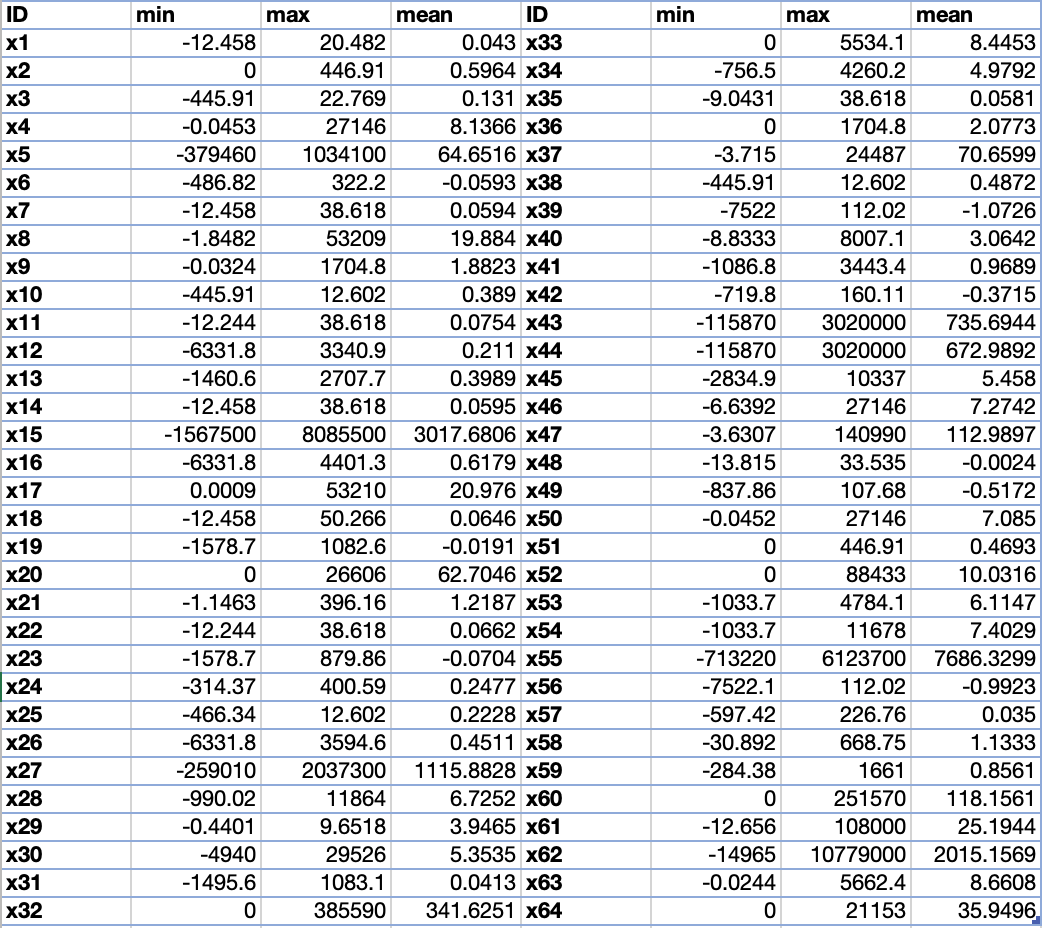
\includegraphics[width=\columnwidth]{Images/y4mmm.png}}
\caption{Min, Max and Mean for Year 4 }
\label{fig:y1mmm}
\end{figure}


\begin{figure}[htp]
\centering
\frame{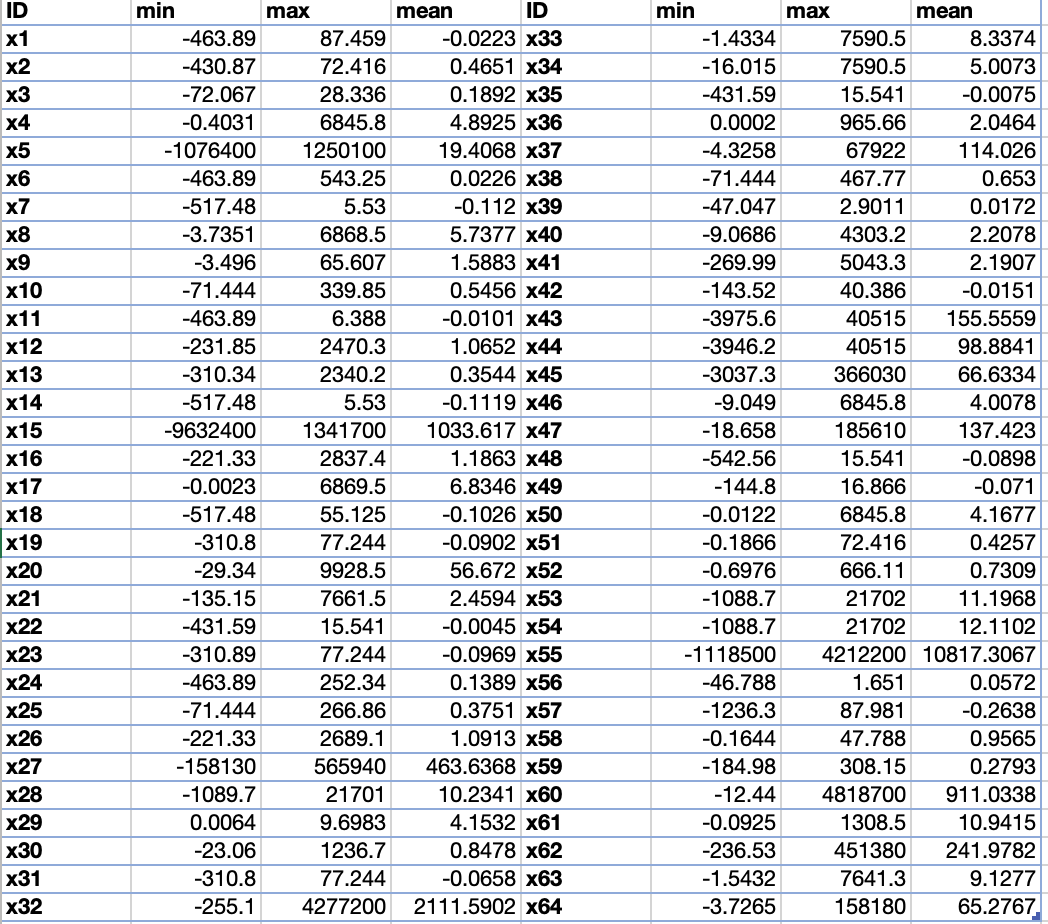
\includegraphics[width=\columnwidth]{Images/y5mmm.png}}
\caption{Min, Max and Mean for Year 5 }
\label{fig:y1mmm}
\end{figure}

